\documentclass[fr,license=none]{../../../eplsummary}

\usepackage{listings}
\usepackage{graphicx}
\usepackage{amsmath}


\lstset{language={Java}}

\hypertitle{Algorithmique numérique}{3}{SINF}{1113}
{Maxime Wets}
{Ramin Sadre}

\section{Représentation des nombres}
Les nombres entiers sont représentés de manière binaire en "Two's complement" dans la plupart des langages de programmation.

\subsection{Représentation Fixed-point}
Dans la représentation fixed-point, un nombre $x$ est repésenté par $2^k * x$. Par exemple :
\begin{itemize}
    \item[-] Addition de $x$ et $y$ : $(2^k * x) + (2^k * y)$
    \item[-] Multiplication de $x$ et $y$ : $(2^k *x) * (2^k * y) / 2^k$
\end{itemize}
Voici une représentation \textbf{fixed-point} sur $16$ bits :
\begin{figure}[!ht]
\centering
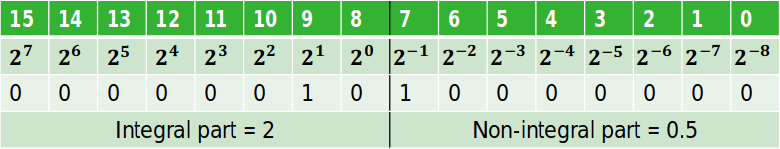
\includegraphics[scale=0.30]{img/fixedpoint.png}
\end{figure}
Avec cette représentation, tous les nombres ne peuvent pas être représentés et la partie décimale a une précision de $\frac{1}{2^k}$. Cette méthode est très facile à implémenter (très facile de décaler des bits). Par contre, si on veut représenter des très grands nombres et des très petits nombres ($10^{10}$ et $10^{-10}$), il faut beaucoup de bits pour la partie entière et pour la partie décimale. C'est donc une méthode très peu efficace.

\subsection{Représentation Floating-point}
L'idée de cette représentation des nombres est de séparer le nombre \textbf{signifiant} de l'\textbf{exposant}. (IEEE 754 décrit le format de cette représentation). Voici comment est stocké un nombre flottant sur $32$ bits dans ce format : \newline
\begin{figure}[!ht]
\centering
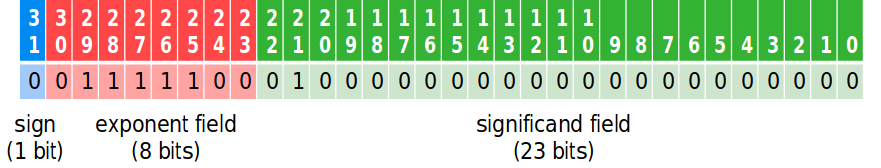
\includegraphics[scale=0.30]{img/ieee754.png}
\end{figure}
La valeur d'un nombre dans le format est donc $(-1)^{b_{31}} * (1.b_{22} \ldots b_0)_2 * 2^{(b_{30} \ldots b_{23})_2 - 127}$. \newline
Cette représentation de nombres est bien plus précise et utilise la mémoire beaucoup plus efficacement que la représentation fixed-point. Cependant, il n'est pas possible de représenter tous les nombres avec ce format. \newline
\begin{figure}[!ht]
\centering
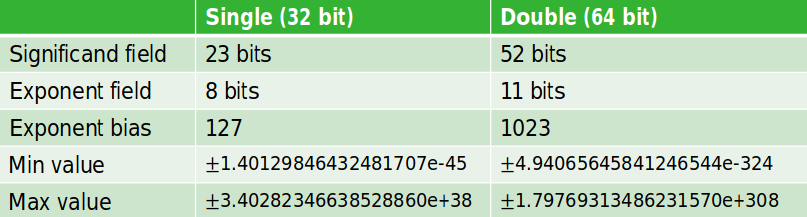
\includegraphics[scale=0.30]{img/ieee754_2.png}
\end{figure}
La précision est finie, les nombres non-représentables sont donc arrondis. Il ne faut donc jamais comparer deux nombres flottants directement. Au lieu de 
\begin{lstlisting}
if (a==b)
\end{lstlisting}
Il vaut mieux utiliser
\begin{lstlisting}
if (Math.abs(a-b) < epsilon)
\end{lstlisting}
avec \emph{epsilon} une valeur arbitraire qui définit la précision (Par exemple : $10^{-16}$)

\subsection{Alternatives}
La \textbf{première alternative} est par exemple la classe \emph{BigDecimal} en Java (les nombres sont représentés dans des chaînes de caractères.
\newline
La \textbf{deuxième alternative} est de représenter les nombres sous forme de fractions de nombres entiers (racket), il n'y a alors pas d'erreur d'approximation. Le point faible est qu'il n'est pas possible de représenter des nombres irrationnels ($\pi$, $\exp$, $\ldots$) et que lorsque l'on additionne deux nombres, il faut trouver le \emph{pgcd} des dénominateurs de ces nombres (qui n'est pas toujours un petit nombre).

\section{Matrices}

\subsection{Représentation de matrices}
Une matrice avec $m$ lignes et $n$ colonnes est représentée comme ça : 
\begin{center}
$$
\begin{pmatrix}
a_{11} & \ldots & a_{1n} \\
\ldots & \ldots & \ldots \\
a_{m1} & \ldots & a_{mn} \\
\end{pmatrix}
$$
\end{center}
Dans la mémoire, les matices sont représentées différemment suivant le langage de programmation. En Java, les matrices sont représentées comme plusieurs plusieurs tableaux unidimensionnels (les blocs de mémoire peuvent se trouver à plusieurs endroits différents en mémoire). En C, les matrices sont représentées de la même manière sauf que les blocs sont continus en mémoire. (Voir \emph{man mmap(2)} pour voir comment récupérer des blocs de mémoire continus grâce à la mémoire virtuelle).

\subsection{Additionner deux matrices}
Mathématiquement, additionner deux matrices $C = A+B$ revient à faire 
$$c_{ij} =  a_{ij} + b_{ij}$$
Pour tous les éléments de $a$ et $b$.

\lstinputlisting{algorithms/mat_addition.java}

% L'algorithme est implémenté dans l'annexe \ref{algos_mat_add}
En pratique, l'ordre des boucles a une importance car les vitesses d'accès en mémoire sont différentes suivant si le bloc se trouve en RAM, cache ou CPU. (Voir Slides 1.18 pour voir pourquoi accéder d'abord aux lignes est plus efficace). Il est beaucoup plus efficace de faire i-j que j-i.

\subsection{Multiplier deux matrices}
Pour multiplier deux matrices $A$ et $B$, on fait
\begin{equation}
    c_{ij} = \sum\limits_{k=1}^m a_{ik}b_{kj}
\end{equation}
Et on obtient comme ça tous les éléments de $C$.
\lstinputlisting{algorithms/mat_multiplication.java}
% L'algorithme est implémenté dans l'annexe \ref{algos_mat_mult}
L'ordre des boucles n'a pas réellement d'importance mais cette implémentation (k-i-j) est bien plus rapide en pratique que (i-j-k).

\subsubsection{Tiling}
Découper des grandes matrices en matrices plus petites permet d'augmenter la localité en mémoire (Voir cours d'élec de première) même si la complexité reste la même ! On peut généralement découper les matrices $n*n$ en deux parties $b*b$ où chaque matrice est de taille $\frac{n}{b}*\frac{n}{b}$. La valeur de $b$ dépend du CPU utilisé, mais voici un exemple de \emph{tiling} où $b = 56$ :
\begin{figure}[!ht]
\centering
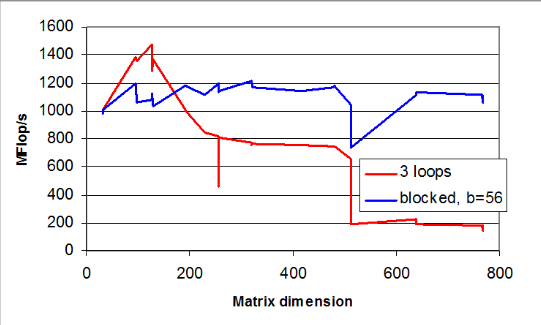
\includegraphics[scale=0.30]{img/tiling.png}
\end{figure}

\subsection{Algorithme de Strassen}
L'algorithme de Strassen tente de de diminuer la complexité de la multiplication de matrices en réduisant le nombre de multiplications. Au lieu de \newline
$$
A*B = 
\begin{pmatrix}
A_{11} B_{11} + A_{12} B_{21} & A_{11} B_{12} + A_{12} B_{22} \\
A_{21} B_{11} + A_{22} B_{21} & A_{21} B_{12} + A_{22} B_{21} \\
\end{pmatrix}
$$
L'algorithme fait 
$$
A*B = 
\begin{pmatrix}
M_1 + M_4 - M_5 + M_7 & M_3 + M_5 \\
M_2 + M_4 & M_1 - M_2 + M_3 + M_6 \\
\end{pmatrix}
$$
\newline
Avec 
\begin{itemize}
    \item[-] $M_1 = (A_{11} + A_{22})(B_{11}+B_{22})$
    \item[-] $M_2 = (A_{21} + A_{22})B_{11}$
    \item[-] $M_3 = A_{11} (B_{12} - B_{22})$
    \item[-] $M_4 = A_{22} (B_{21} - B_{11})$
    \item[-] $M_5 = (A_{11} + A_{12}) B_{22}$
    \item[-] $M_6 = (A_{21} - A_{11}) (B_{11} + B_{12})$
    \item[-] $M_7 = (A_{12} - A_{22}) (B_{21} + B_{22})$
\end{itemize}
On ne fait donc que $7$ multiplications (une multiplication est plus "chère" qu'une addition : Voir cours d'élec de première) donc la complexité est de $O(2^{2.81})$ pour pour l'algorithme de Strassen. \newline
En pratique, la multiplication en utilisant un algorithme de \textbf{tiling} est bien plus efficace, même si la complexité reste cubique.

\subsection{Shape-based optimizations}
Il arrive qu'une matrice contienne beaucoup de $0$, stocker cette matrice en mémoire est donc très inefficace, il existe plusieurs solutions pour remédier à ce problème. Attention : si on utilise cette optimisation pour la représentation de matrices, il faut adapter les algorithmes de manipulation de matrices !

\subsection{Sparse matrices}
Une \textbf{sparse matrix} est une matrice très grande où la plupart des entrées est $0$, on peut les représenter comme 
\begin{itemize}
    \item[-] une table de hachage : 
    \begin{lstlisting}
    HashMap m = new Hashmap();
    m.put(new Location(5,8), 34.3);
    \end{lstlisting}
    
    \item[-] une liste d'entrées :
    \begin{lstlisting}
    LinkedList m = new LinkedList();
    m.add(new Entry(5,8, 34.3);
    \end{lstlisting}

    \item[-] un tableau compressé :
    \begin{lstlisting}
    double[][] m = new double[][] {
        {3, 4.0, 0, 5.0, 5, 1.0}, // ligne 1
        {0, 2.0, 10} // ligne 2
    }
    \end{lstlisting}
    Ce qui signifie que 
    \begin{itemize}
        \item[$\to$] Ligne 1 = $\{0,0,0,4,5,0,0,0,0,0,1\}$
        \item[$\to$] Ligne 2 = $\{2,0,0,0,0,0,0,0,0,0,0\}$
    \end{itemize}
\end{itemize}

\section{Systèmes linéaires}

\subsection{Elimination de Gauss-Jordan}
L'élimintation de Gauss-Jordan permet d'obtenir une matrice échelonnée (réduite). Pour résoudre un sytème $AX = B$, on va
\begin{enumerate}
    \item Faire des \textbf{forward substitutions} jusqu'à obtenir une matrice triangulaire supérieure
    $$
    \begin{pmatrix}
    1 & X & X & | & X \\
    0 & 1 & X & | & X \\
    0 & 0 & 1 & | & X \\
    \end{pmatrix}
    $$
    
    \item Faire des \textbf{backward substitutions} jusqu'à obtenir
    $$
    \begin{pmatrix}
    1 & 0 & 0 & | & X \\
    0 & 1 & 0 & | & X \\
    0 & 0 & 1 & | & X \\
    \end{pmatrix}
    $$
\end{enumerate}
L'algorithme pour effectuer une \textbf{forward substitution} est 
\begin{enumerate}
    \item Choisir un pivot.
    \item Diviser toute la ligne par le pivot.
    \item Eliminer les valeurs en dessous du pivot.
    \item Répéter les étaples précédentes avec la ligne suivante.
\end{enumerate}
La résultat est une matrice triangulaire supérieure.
\newline
L'algorithme pour effectuer une \textbf{backward substitution} est très similaire au \textbf{forward substitution} puisqu'il fait l'inverse, jusqu'à obtenir une matrice diagonale.

\subsubsection{Complexité de la méthode de Gauss}
L'élimination de Gauss utilise trois types d'opérations 
\begin{enumerate}
    \item Permuter les lignes
    \item Multiplier tous les éléments d'une ligne par le pivot
    \item Eliminer une ligne
\end{enumerate}
Pour une matrice $n*n$, chaque opération a une complexité en $O(n)$. Vu qu'il y a $n$ \emph{forward} et \emph{backward substitutions}, la complexité finale de l'algorithme est en $O(n^3)$.

\subsubsection{Stabilité numérique de la méthode de Gauss}
Dans le premier chapitre sur la \underline{représentation des nombres}, on a vu que tous les nombres \textbf{floating-point} ne sont pas représentables. Si le pivot est une valeur minuscule (très proche de $0$ mais pas $0$), il peut y avoir des erreurs de calcul dues à la précision finie. De fait, un bon pivot est un pivot dont la valeur absolue est très grande. \newline
Pour choisir un bon pivot, il y a deux méthodes :
\begin{enumerate}
    \item \textbf{Partial pivoting}
    \item \textbf{Full Pivoting}
\end{enumerate}
Le \textbf{partial pivoting} consiste en échanger des linges afin de trouver le pivot le plus grand possible, par exemple :
\begin{figure}[!ht]
\centering
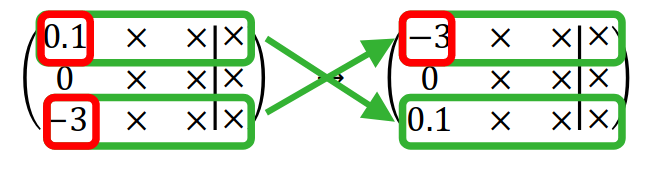
\includegraphics[scale=0.25]{img/partialpivoting.png}
\end{figure}
Pour le \textbf{full pivoting}, on cherche dans toute la matrice le pivot le plus grand possible et on échange les lignes et/ou les colonnes. Cela donne un meilleur résultat (bien que ce soit plus long à calculer). Attention : échanger les colonnes change l'ordre des variables, il faut donc se souvenir des changements.
\begin{center}
    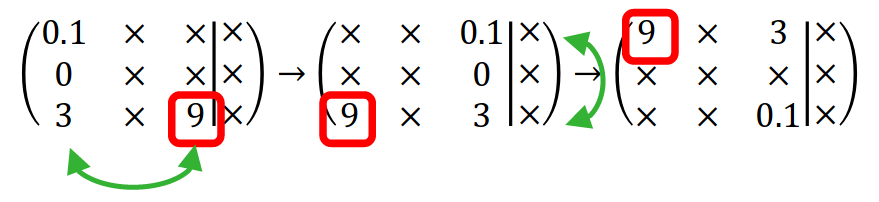
\includegraphics[scale=0.25]{img/fullpivoting.png}
\end{center}

\subsubsection{Résoudre plusieurs problèmes simultanément}
Vu que pour résoudre un système $AX = B$, les étapes de l'élimination de Gauss ne dépendent que de $A$ et pas de $B$, il est possible de résoudre deux systèmes $AX_1 = B_1$ et $AX_2 = B_2$ simultanément, puisque $(A|B_1)$ et $(A|B_2)$ requièrent les mêmes manipulations pour trouver $X_1$ et $X_2$. (Voir Slides 3.20 pour l'exemple). Cela peut servir à trouver des matrices inverses facilement car dans la plupart des problèmes, il faut calculer des inverses de la forme $C = A^{-1}B$, on peut donc trouver $C$ en résolvant le système $AC = B$.
% L'algorithme est implémenté dans l'annexe \ref{algos_syslin_gauss}

\subsection{Méthode LU Decomposition}
La méthode du LU Decomposition est une autre manière de trouver les solutions d'un système $AX = B$. Il s'agit en fait de décomposer la matrice $A$ en une matrice triangulaire inférieure $L$ et une matrice triangulaire supérieure $U$. De sorte que
\begin{figure}[!ht]
\centering
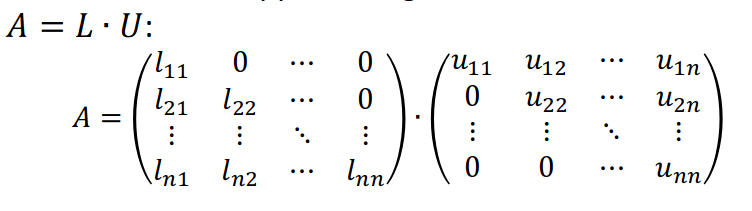
\includegraphics[scale=0.30]{img/ludecomposition.png}
\end{figure}
L'avantage de cette méthode est qu'on peut résoudre le système en faisant $L U X = B$ où on peut utiliser $L Y = B$ pour trouver $Y = U X$. La complexité pour trouver $L$ et $U$ est $O(n^3)$ (élimination de Gauss) mais l'avantage est qu'une fois qu'on a $L$ et $U$ pour $A$ on n'a plus à les calculer et on peut résoudre le système $L U X = B$ pour tout $B$ (pratique lorsqu'il faut résoudre le système pour plusieurs matrices $B_i$ différentes).
% L'algorithme est implémenté dans l'annexe \ref{algos_syslin_lud}

\subsection{Méthode de Jacobi}

La méthode de Jacobi est une solution itérative pour trouver une solution à système de matrices $AX = B$. D'abord, il faut séparer la matrice A en deux sous-matrices D et R. \newline
$D := $ la matrice contenant uniquement les éléments diagonaux de A \newline
$R := $ la matrice contenant tous les éléments de A sauf les éléments diagonaux
La méthode de Jacobi utilise la formule d'itération suivante :
\newline
$X^{(0)} := $ approximation initiale \newline
$X^{(k + 1)} := D^{-1}(B - RX^{(k)})$ \newline
Mathématiquement, on peut écrire cette formule : \newline
\begin{equation}
    x_{i}^{(k+1)} := \frac{1}{a_{ii}} (b_i - \sum\limits_{j \neq i} a_{ij}x_j^{(k)}), i = 1, 2, \ldots, n
\end{equation}
L'algorithme pour implémenter la méthode de Jacobi est le suivant :
\begin{enumerate}
    \item Choisir une estimation initiale $X^{(0)}$, $k := 0$
    \item A partir de $X^{(k)}$, calculer la nouvelle estimation $X^{(k+1)}$: \newline
        $x_{i}^{(k+1)} := \frac{1}{a_{ii}} (b_i - \sum\limits_{j \neq i} a_{ij}x_j^{(k)})$ , $i = 1, 2, \ldots, n$
    \item Répéter l'étape 2 jusqu'à convergence : difference($X^{(k+1} - X^{(k)}$)$ < \epsilon$
    \item L'erreur est égale à $AX^{(k+1)} - B$
\end{enumerate}

Dans la troisième étape, difference($X$, $Y$) peut être
\begin{itemize}
    \item $max_{i}|x_i - y_i|$
    \item $\sum\limits_i (x_i - y_i)^2$
\end{itemize}
Parfois, l'algorithme s'arrête trop tôt parce que $X^{(k)}$ et $X^{(k+1}$ sont très proche mais $X^{(k+2)}$ est beaucoup mieux. Pour pallier à ce problème, on peut utiliser difference($X^{(k+1} - X^{(k-1)}$) à la place. \newline
Le problème avec la méthode de Jacobi est que la solution ne converge pas toujours. Une condition suffisante (mais pas nécessaire) pour vérifier la convergence est $$|a_{ii}| > \sum\limits_{j \neq i}|a_{ij}|$$

\subsection{Méthode de Gauss-Seidel}
La méthode de Gauss-Seidel est une variante de la méthode de Jacobi : on utilise le $x_{i..i-1}^{(k+1)}$ calculé précédemment pour calculer $x_i^{(k+1)}$
\begin{equation}x_i^{(k+1)} := \frac{1}{a_{ii}} (b_i - \sum\limits_{j=1}^{i-1} a_{ij}x_j^{(k+1)} - 
\sum\limits_{j=i+1}^n a_{ij}x_j^{(k)} )
\end{equation}
La rapidité de cette solution dépend de A et peut être plus rapide ou plus lente que la méthode de Jacobi. \newline
\textbf{Point positif : } Un seul vecteur $X^{(k)}$ doit être stocké. \newline
\textbf{Point négatif : } Ne peut pas être parallélisé parce que le calcul de $x_{i}^{(k+1)}$ a besoin de  $x_{i-1}^{(k+1)}$, $x_{i-2}^{(k+1)}$, etc. \newline
% L'algorithme est implémenté dans l'annexe \ref{algos_syslin_gauss_seidel} :

\section{Régression linéaire}

\subsection{Introduction}
Le problème de la régression linéaire est le suivant : il faut trouver les coefficients $a_{i}$ pour le système suivant.
$$
\begin{pmatrix}
x_1^{(1)} & x_2^{(1)} & \ldots & x_n^{(n)} \\
\ldots & \ldots & \ldots & \ldots \\
x_1^{(m)} & x_2^{(m)} & \ldots & x_n^{(m)} \\
\end{pmatrix}
\quad
\begin{pmatrix}
a_1 \\
\ldots \\
a_n \\
\end{pmatrix}
\quad
=
\begin{pmatrix}
y^{(1)} \\
\ldots \\
y^{(m)} \\
\end{pmatrix}
\quad
$$
\newline
Si $m = n$, on a une matrice carrée et c'est donc très simple à résoudre, cependant, il est courant d'avoir $m > n$ et alors on a trop de données pour trouver la solution. (Noter que les coefficients $a_i$ sont les inconnues).

\subsection{Least-Square method}
La méthode des \textbf{Least-Square} essaie de minimiser $|| Y - XA||_2$ pour $|| (v_1 \ldots v_n)||_2 = \sqrt{\Sigma_{i=1}^nv_i^2}$. On peut noter que minimiser  $|| Y - XA||_2$ est la même chose que de minimiser  $|| Y - XA||_2^2$. \newline
Les équations normales $X^TXA = X^TY$ ont une solution unique pour ce système si il y a au moins $n$ lignes de $X$ qui sont linéairement indépendantes. (Voir Slides 4.9 pour la démonstration)

\subsection{Régression polynomiale}
Au lieu d'utiliser $f(x) = a_1 + a_2x$, on peut utiliser le modèle polynomial : $f(x) = a_1 + a_2x + a_3x^2 + \ldots + a_nx^{n-1}$. Avec un système
$$
\begin{pmatrix}
1 & x^{(1)} & (x^{(1)})^2 & \ldots & (x^{(1)})^{n-1} \\
\ldots &\ldots & \ldots & \ldots & \ldots \\
1 & x^{(m)} & (x^{(m)})^2 & \ldots & (x^{(m)})^{n-1} \\
\end{pmatrix}
\quad
\begin{pmatrix}
a_1 \\
\ldots \\
a_n \\
\end{pmatrix}
\quad
=
\begin{pmatrix}
y^{(1)} \\
\ldots \\
y^{(m)} \\
\end{pmatrix}
\quad
$$
On peut toujours utiliser la méthode \textbf{Least-Square} pour trouver $A$. Les équations normales $X^TXA = X^TY$ restent correctes  et $X$ est appelée la \textbf{matrice de Vandermonde}.

\subsection{Factorisation de Cholesky}
La factorisation de Cholesky concerne les matrices SPD (symmetric positive definite matrices) qui sont très courantes dans les problèmes numériques. Pour une matrice $C$ qui est SPD, il existe une factorisation unique $C = LL^T$ où $L$ est une matrice triangulaire inférieure. Une fois qu'on connait $L$, un système linéaire $CX = B$ peut être résolu en $O(n^2)$. Cela peut être comparé à la \textbf{LU Decomposition} sauf qu'il suffit d'une seule matrice. \newline
Pour calculer $L$, on a \newline
\begin{figure}[!ht]
\centering
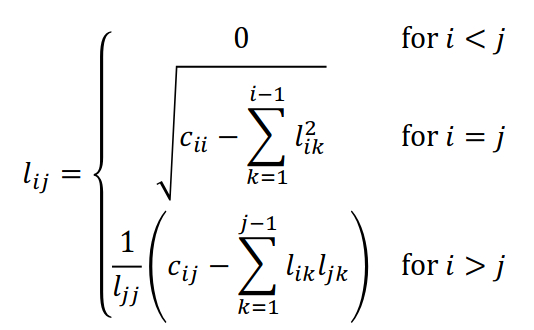
\includegraphics[scale=0.40]{img/computation_L.png}
\end{figure}
Cette méthode a une complexité en $O(n^3)$ mais en pratique cette méthode est bien plus rapide que la \textbf{LU Decomposition} parce qu'une seule matrice $L$ doit être calculée.
% L'algorithme est implémenté dans l'annexe \ref{algos_reglin_cholesky}

\section{Normes et conditions des matrices}

\subsection{Est-ce que les équations normales sont un problème "facile" ?}
Avec la méthode \textbf{Least-Square}, on a vu que les systèmes $XA \approx B$ peut être résolu en en résolvant les \textbf{équations normales} $X^T XA = X^T Y$. En pratique, l'erreur devient trop grande lorsque $X$ a des colonnes \emph{presque} linéairement dépendantes.

\subsection{Qualité d'une matrice}
Pour exprimer mathématiquement la qualité d'une matrice, il faut d'abord voir ce qu'est une norme d'un vecteur et une norme de matrice.

\subsubsection{Norme d'un vecteur}
La norme d'un vecteur est la fonction $||.||: R^n \rightarrow [0, \inf$ 
Où 
\begin{itemize}
    \item[-] $||V|| = 0$ si et seulement si $V = 0$
    \item[-] $||cV|| = |c| . ||V||$ pour tout $c \in R$
    \item[-] $||V+W|| \leq ||V|| + ||W||$ (égalité triangulaire).
\end{itemize}
Il existe plusieurs types de normes de vecteurs:
\begin{itemize}
    \item[-] \textbf{1-norm} (ou norme de \emph{Manhattan}): \newline
    $||(v_1 \ldots v_n)||_1 = \sum\limits_{i=1}^n |v_i|$
    \item[-] \textbf{2-norm}: \newline
    $||(v_1 \ldots v_n)||_2 = \sqrt{\sum_{i=1}^n v_i^2}$
    \item[-] \textbf{$\inf$-norm}: \newline
    $||(v_1 \ldots v_n)||_{\inf} = \max |v_i|$
\end{itemize}
Il peut être démontré que toutes les normes de vecteurs sont plus ou moins équivalentes : \newline
Pour deux normes $||.||$ et $||.||^{'}$, il existe toujours deux constantes $a, b \in R$ telles que $a||V|| \leq ||V||^{'} \leq b||V|| \forall V$

\subsubsection{Norme de matrice}
Une norme de matrice $||A||$ dans $R^{m*n}$ est induite par une norme de vecteur $||V||$ si \newline
$||A|| = \max\limits_{V \neq 0} \frac{||AV||}{||V||} = \max_{||V|| = 1} ||AV||$ \newline
A nouveau, suivant la norme de $V$, la norme de la matrice sera légèrement différente : 
\begin{itemize}
    \item[-] Norme de matrice induite par $||V||_1$: \newline
    $||A||_1 = \max\limits_{1 \leq j \leq n} \sum\limits_{i=1}^m |a_{ij}|$
    \item[-] Norme de matrice induite par $||V||_2$: \newline
    $||A||_2 = \sqrt{largest eigenvalue of A^TA}$
    \item[-] Norme de matrice induite par $||V||_{\inf}$: \newline
    $||A||_{\inf} = \max\limits_{1 \leq i \leq m} \sum\limits_{j=1}^n |a_{ij}|$
\end{itemize}
Les normes de matrices induites sont \emph{sub-multiplicative} : $||A . B|| \leq ||A|| . ||B||$ \newline (Cette propriété est utile pour les preuves mathématiques).

\subsection{Perturbation d'un système linéaire}
On s'intéresse à la taille de l'erreur relative d'une solution lorsque le système est perturbé par une petite erreur $\epsilon$ : \newline
$\frac{||X(\epsilon) - X(0)||}{||X(0)||} = $ ? \newline
Après des calculs (Voir Slides 5.16-17), on obtient l'inégalité suivante : \begin{equation}
\frac{||X(\epsilon) - X(0)||}{||X(0)||} = \leq |\epsilon| (\frac{||\delta B||}{||B||} + \frac{||\delta A||}{||A||}) ||A|| * ||A^{-1}|| + O(\epsilon^2)
\end{equation}
Pour toute norme de matrice induite $||.||$.

\subsubsection{Matrix condition number}
On définit la \textbf{Matrix condition number} (pour une norme $||.||$) comme $cond A = ||A||*||A^{-1}||$. Plus $cond A$ est grand, plus la solution de $AX = B$ est sensible aux perturbations. (On dit que $A$ et $AX = B$ sont \textbf{ill-conditioned}).\newline 
Pour voir si un système $AX = B$ est stable, on pourrait d'abord calculer $cond A$ et ensuite résoudre le système. Seul problème : calculer $||A^{-1}||$ peut être aussi complexe que de résoudre $AX = B$ (on aurait donc besoin d'un \emph{condition number} pour calculer le \emph{condition number}). \newline
En pratique, on essaie de calculer les bornes de $cond A$ pour voir les performances d'un algorithme dans le meilleur/pire cas.

\subsection{Equations normales}
Pour revenir à la première question du chapitre (Est-ce que les équations normales sont un problème "facile" ?) $X^T XA = X^T Y$. Si on calcule la \emph{condition number} de $X^T X$, on obtient $cond X^T X = (cond X)^2$, donc $X$ est \textbf{ill-conditioned}, $X^T X$ est donc encore pire (Voir Slides 5.21). \newline
A cause de ça, les bonnes implémentations de l'algorithme \textbf{Least-Square} ne résolvent pas directoement $X^T XA = X^T Y$, ils utilisent à la place le \textbf{QR factorization} qui factorisent les matrices $X^T X = QR$ (où $R$ est une matrice triangulaire).

\section{Interpolation}

\subsection{Introduction}
Le but de l'interpolation est de trouver une fonction $f(x_1^{i}, x_2^{(i)}, \ldots, x_n^{(i)} = y^{(i)})$ pour $i = 1, 2, \ldots, m$. Ce n'est donc pas la même chose que la régression linéaire dans le sens où $f$ est plus "plate"

\subsection{Interpolation polynomiale}
On utilise la fonction $f(x) = a_1 + a_2x + a_3x^2 + \ldots + a_nx^{n-1}$ pour l'interpolation polynomiale. On peut trouver les $a_i$ en résolvant le système de Vandermonde
$$
\begin{pmatrix}
1 & x^{(1)} & (x^{(1)})^2 & \ldots & (x^{(1)})^{n-1} \\
\ldots &\ldots & \ldots & \ldots & \ldots \\
1 & x^{(m)} & (x^{(m)})^2 & \ldots & (x^{(m)})^{n-1} \\
\end{pmatrix}
\quad
\begin{pmatrix}
a_1 \\
\ldots \\
a_n \\
\end{pmatrix}
\quad
=
\begin{pmatrix}
y^{(1)} \\
\ldots \\
y^{(m)} \\
\end{pmatrix}
\quad
$$
Si $n = m$ et que toutes les lignes sont linéairement indépendantes, alors le rang de la matrice est $n$ et la matrice a une solution unique. La complexité de la méthode de Vandermonde est de $O(n^3)$ mais elle ne fonctionne pas très bien lorsque le nombre de points augmente. Cela veut dire que les colonnes de droite de la matrice à gauche dans le calcul deviennent très similaires lorsque $n$ augmente, ce qui fait que le système devient numériquement instable.
\begin{figure}[!ht]
\centering
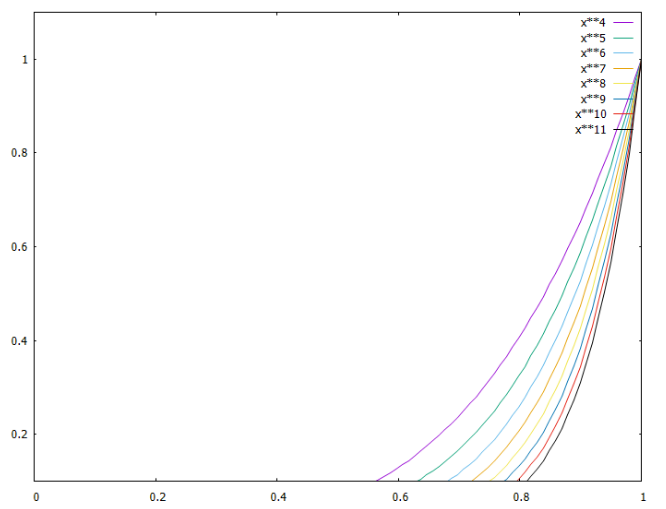
\includegraphics[scale=0.40]{img/vandermonde_problem.png}
\end{figure}

\subsection{Interpolation de Lagrange}
La formule de l'interpolation de Lagrange est :
\begin{equation}
f(x) = \sum\limits_{i=1}^n y^{(i)}\phi_i(x)
\end{equation}
avec $\phi_i(x)$ une fonction simple. La méthode de Lagrange utilise
$$\phi_i(x) = \frac{\prod_{j \neq i}(x - x^{(j)})}{\prod_{j \neq i}(x^{(i)} - x^{(j)})}$$

Les $\phi(x)$ sont donc les polynômes de degré $n-1$. Le résultat obtenu est le même que si l'on résout $XA = Y$ sauf que $\phi_i(x)$ peut être obtenu directement de la définition. (Il n'est donc pas nécessaire de résoudre $XA = Y$).

\subsubsection{Propriétés}
\begin{itemize}
    \item[-] \textbf{Complexité : } $O(n^2)$
    \item[-] \textbf{Point positif : } On n'a pas le problème de résoudre $AX = Y$ donc la complexité n'augmente pas comme sur le graphe.
    \item[-] \textbf{Point positif : } Une fois qu'on connait les $\phi_i(x)$, il est très facile de calculer $f(x)$ pour différents $y^(i)$
    \item[-] \textbf{Point négatif : } Si $x^{(1)}, x^{(2)}$ sont très proches, le calcul de $\phi_i(x) = \frac{\prod_{j \neq i}(x - x^{(j)}}{\prod_{j \neq i}(x^{(i)} - x^{(j)}}$ implique une division par un produit de très petites valeurs, ce qui implique qu'en pratique, cette méthode n'est pas utilisée en pratique.
\end{itemize}

\subsection{Interpolation de Newton}
La formule de l'interpolation de Newton est :
\begin{equation} 
f(x) = \sum\limits_{i=1}^n c_i \psi_i(x)
\end{equation} 
avec la base de Newton
$$\psi_i(x) = \prod_{j=1}^{i-1}(x - x^{(j)}$$
Pour trouver les $c_i$, il faut résoudre le système
$$
\begin{pmatrix}
\psi_1(x^{(1)}) & 0 & 0 & \ldots & 0 \\
\psi_1(x^{(2)}) & \psi_2(x^{(2)}) & 0 & \ldots & 0 \\
\ldots & \ldots & \ldots & \ldots & \ldots \\
\end{pmatrix}
\begin{pmatrix}
c_1 \\
\ldots \\
c_n \\
\end{pmatrix}
=
\begin{pmatrix}
y^{(1)} \\
\ldots \\
y^{(m)} \\
\end{pmatrix}
$$
C'est une matrice triangulaire inférieure, ce système est donc facile à résoudre.

\subsubsection{Propriétés}
\begin{itemize}
    \item[-] \textbf{Complexité : } $O(n^2)$
    \item[-] \textbf{Point positif : } Numériquement stable
    \item[-] \textbf{Point positif : } Ajouter un nouveau point $(x^{(n+1}, y^{(n+1)})$ n'implique pas de devoir tout recalculer.
\end{itemize}

\subsection{Erreur d'interpolation}
Si on définit $g(x)$ la fonction polynomiale qui a interpolé $f(x)$ avec $n$ points, l'erreur d'interpolation est $e(x) = g(x) - f(x)$. Le problème est que pour certaines fonctions (Par exemple : $\frac{1}{1 + x^2}$), l'erreur augmente de plus en plus lorsque n tend vers l'infini et que les points à interpoler sont équidistants. Il peut être démontré qu'il existe $\xi \in ]x^{(1)}, x^{(n)}[$ pour chaque $x \in ]x^{(1)}, x^{(n)}[$ tel que
\begin{equation} 
e(x) = \frac{g^{(n)} (\xi(x))}{n!} \prod\limits_{i=1}^n (x - x^{(i)})
\end{equation}
si $g(x)$ est continué et $n$ fois différentiable sur $]x^{(1)}, x^{(n)}[$

\subsubsection{Points de Chebyshev}
Pour une fonction $g(x)$ défini sur l'intervalle $[-1,1]$, $e(x)$ est minimisée si on choisit les points 
$$x^{(i)} = cos(\frac{2i-1}{2n}\pi)$$
pour $i = 1, \ldots, n$ \newline
Pour les fonctions définies sur l'intervalle $[a,b]$, on peut étendre cette propriété : 
\begin{equation}
x_{[a,b]}^{(i)} = \frac{a+b}{2} + \frac{b - a}{2} x^{(i)}
\end{equation}

\section{Splines}

\subsection{Cubic Splines}

\subsubsection{Interpolation parfaite ?}
Le théorème d'approximation de \textbf{Weierstrass} dit :
\begin{center}
    Soit $g(x)$, une fonction continue sur $[a,b]$. Pour chaque $\epsilon > 0$, il existe un polynôme $f(x)$ tel que $||g-f||_{\inf} < \epsilon$ dans l'intervalle $[a,b]$.
\end{center}
En pratique, ce n'est pas toujours pratique car avoir des polynômes avec un degré trop haut complique les calculs.

\subsubsection{Piecewise interpolation}
L'interpolation par morceaux prend $n$ points d'une fonction et approxime $g(x)$ par une fonction $f(x)$ qui consiste en $n-1$ polynômes de degré identique, chacun interpolant une partie de $g(x)$. \newline
Avec des constantes : 
\begin{figure}[!ht]
\centering
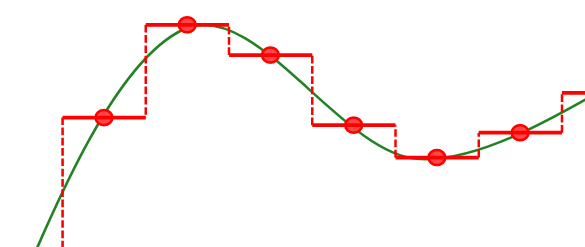
\includegraphics[scale=0.25]{img/piecewise_const.png}
\end{figure}
Linéairement :
\begin{figure}[!ht]
\centering
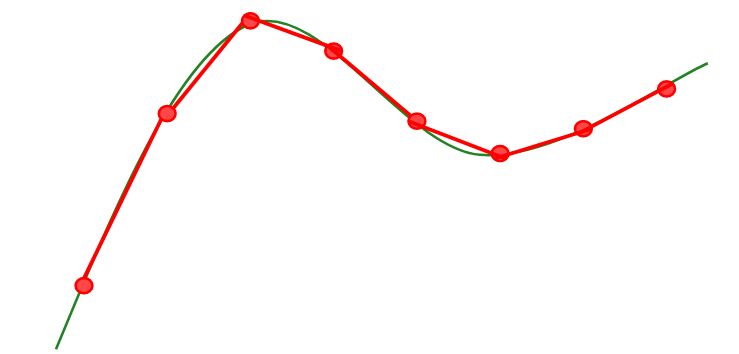
\includegraphics[scale=0.20]{img/piecewise_linear.png}
\end{figure}

\subsubsection{Cubic spline}
Une \textbf{cubic spline} utilise des polynômes de degré $3$ pour interpoler les intervalles $[x^{(i)}, x^{(i)}]$ entre les points $(x^{(i)}, y^{(i)})$ et $(x^{(i+1)}, y^{(i+1)})$, mais il y a un nombre infini de polynômes de degré $3$ entre les deux points ! Il faut choisir le polynôme cubique de sorte que la \textbf{spline} finale $f(x)$ soit deux fois différentiable.
\newline
Pour les points $(x^{(i)}, y^{(i)})$ et $(x^{(i+1)}, y^{(i+1)})$, il faut essayer de trouver un polynôme de degré $3$ $s_i (x)$ tel que 
\begin{itemize}
    \item[-] $s_i (x^{(i)}) = y^{(i)}$
    \item[-] $s_{i-1} (x^{(i)}) = y^{(i)}$
\end{itemize}
Et il faut également que $x^{(i)}$ soit deux fois différentiable de sorte que : 
\begin{itemize}
    \item[-] $s_i^{'} (x^{(i)}) = s_{i-1}^{'} (x^{(i)})$
    \item[-] $s_i^{''} (x^{(i)}) = s_{i-1}^{''} (x^{(i)})$
\end{itemize}
Graphiquement, ça donne ça :
\begin{figure}[!ht]
\centering
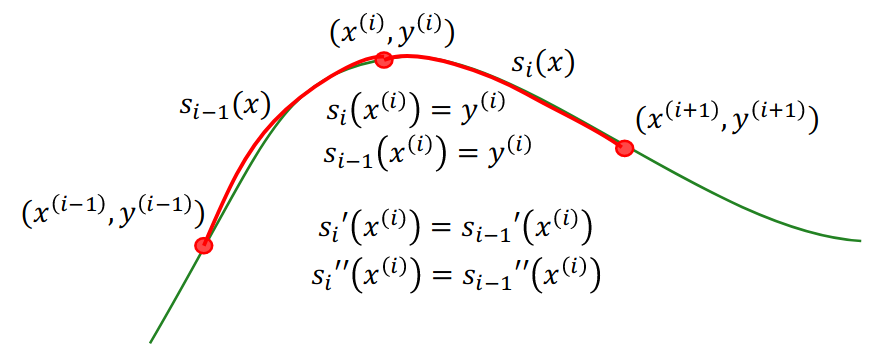
\includegraphics[scale=0.25]{img/cubicsplines.png}
\end{figure}
En général, les polynômes d'ordre $3$ sont représentés comme :
$$s_i(x) = a_i + b_i(x-x^{(i)}) + c_i(x-x^{(i)})^2 + d_i(x-x^{(i)})^3$$
avec
$$s_i^{'}(x) = b_i + 2c_i(x-x^{(i)}) + 3d_i(x-x^{(i)})^2$$
$$s_i^{''}(x) = 2c_i + 6d_i(x-x^{(i)})$$

En mettant toutes les équations ensemble, on obtient
\begin{equation}
    c_{i-1}(x^{(i)} - x^{(i-1)}) + 2c_i (x^{(i+1)} - x^{(i-1)}) + c_{i+1}(x^{(i+1)} - x^{(i)})
\end{equation}
C'est donc un système de $n-2$ équations à $n$ inconnues ($c_1, \ldots, c_n$). Pour pouvoir résoudre ce système, on pose $c_1 = c_n = 0$. 

\subsection{B-Splines}
Il existe trois problèmes majeurs à l'interpolation : 
\begin{enumerate}
    \item Changer un point change toute la courbe. Par exemple :
		\begin{figure}[!ht]
		\centering
    	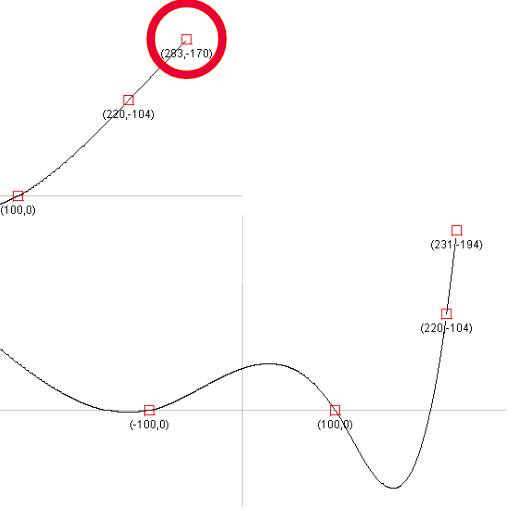
\includegraphics[scale=0.20]{img/drawback1_interpol.png}
		\end{figure}
    \item L'approximation peut diverger fortement des points. Par exemple : 
    \begin{center}
        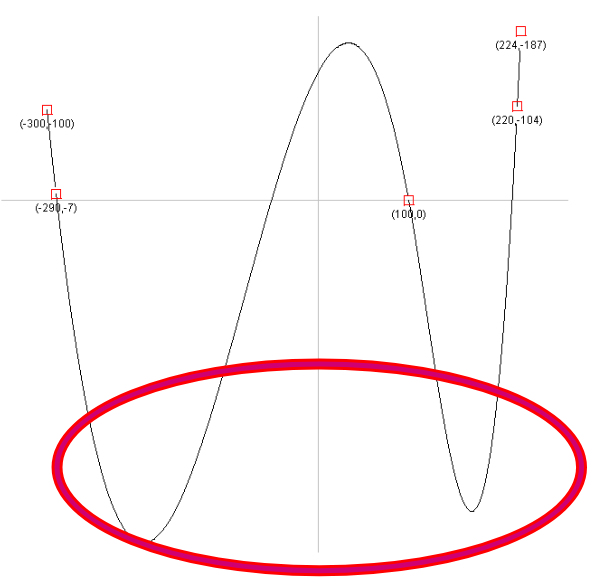
\includegraphics[scale=0.20]{img/drawback2_interpol.png}
    \end{center}
    \item Il est impossible d'interpoler une courbe qui est une fonction de $x$. Par exemple : 
		\begin{figure}[!ht]
		\centering
		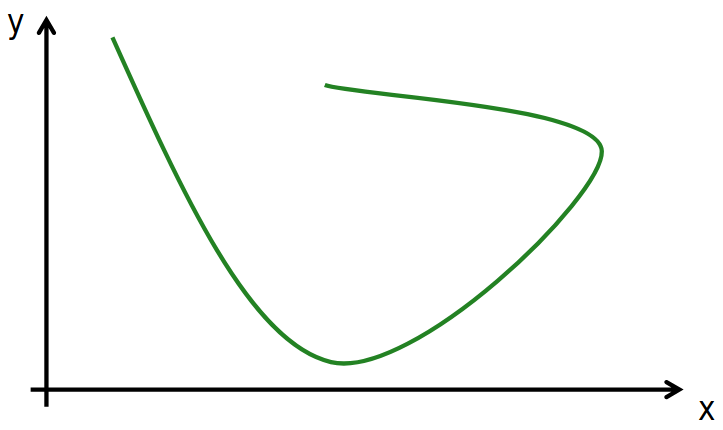
\includegraphics[scale=0.20]{img/drawback3_interpol.png}
		\end{figure}
\end{enumerate}
Avec les \textbf{B-Splines}, 
\begin{enumerate}
    \item Les points ont une influence \emph{locale} sur la courbe.
    \item La courbe ne diverge pas trop des points.
    \item Les \textbf{B-Splines} sont des courbes paramétriques de la forme $x(t), y(t)$. Pas des fonctions telles que $y = f(x)$
\end{enumerate}
Une courbe paramétrique sont décrites par des équations paramétriques. \newline Par exemple, un cercle de rayon $r$ qui est défini par $x(t) = r * \cos(t)$, $y(t) = r * sin(t)$ avec $t \in [0, 2\pi]$
\begin{center}
    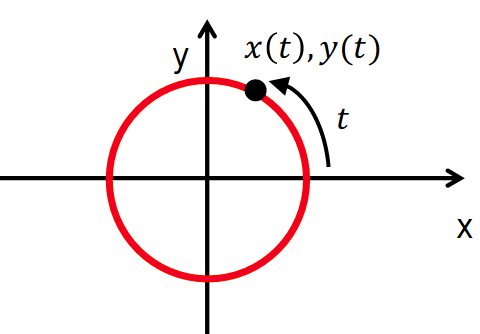
\includegraphics[scale=0.30]{img/circle.png}
\end{center}
Une courbe \textbf{B-Spline} de degré \emph{m} est une combinaison linéaire des fonctions
\begin{equation}
    x(t) = \sum\limits_{i=0}^{n-1}x^{(i)}B_i^m (t)
\end{equation}
\begin{equation}
    y(t) = \sum\limits_{i=0}^{n-1}y^{(i)}B_i^m (t)
\end{equation}
Où
\begin{equation}
    B_i^m (t) = \frac{t - t_i}{t_{i+m} - t_i}B_i^{m-1}(t) + \frac{t_{i+m+1} - t}{t_{i+m+1} - t_{i+1}}B_{i+1}^{m-1}(t)
\end{equation}
Pour choisir les $t_i$ (les noeuds) :
\begin{itemize}
    \item[-] $t_i = 0 $ pour $i \leq m$
    \item[-] $t_i = n-m$ pour $i \geq n$
    \item[-] $t_i = i-m $ autrement
\end{itemize}

\section{Intégration numérique}
\label{intnum}

\subsection{Méthode de Riemann}
La méthode de Riemann définit le calcul d'intégrales comme suit :
\begin{equation}
\int_a^b f(x)dx = \lim\limits_{\Delta k \rightarrow 0} \sum\limits_k f(x_k^{'})(x^{(k+1)} - x^{(k)})
\end{equation}
Où
\begin{itemize}
    \item[-] $a = x^{(1)} < \ldots < x^{(n)} = b$
    \item[-] $\Delta x_k = x^{(k+1)} - x^{(k)}$
    \item[-] $x_k^{'}$ est un point dans l'intervalle $[x^{(k)}, x^{(k+1)}]$
\end{itemize}
Voici une interprétation géométrique de l'intégrale de Riemann :
\begin{figure}[!ht]
\centering
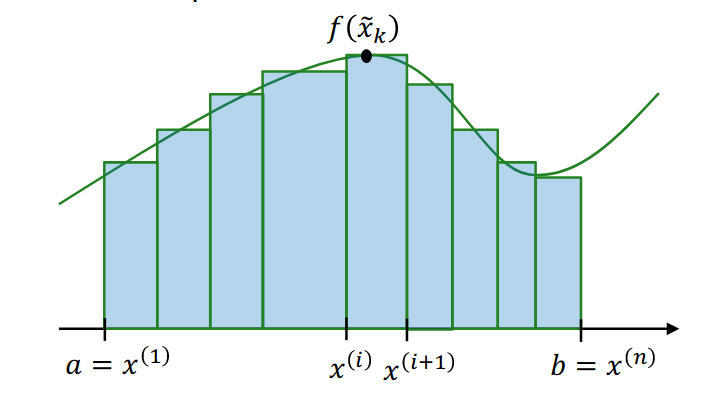
\includegraphics[scale=0.30]{img/riemann_interpretation.png}
\end{figure}
Cependant, pour certaines fonctions, il faut un $\Delta x_k$ très petit pour obtenir une bonne approximation. En pratique, il est très compliqué de calculer $f(x)$ pour beacoup de points et il se peut également que $f(x)$ ne soit connue que pour quelques points. Cette méthode n'est donc pas très utilisée.

\subsection{Quadrature interpolatoire}
L'idée est très similaire au problème de l'interpolation :
\begin{enumerate}
    \item Choisir les points $a \leq x^{(1)} < x^{(2)} < \ldots < x^{(n)} \leq b$
    \item Approximer $f(x)$ en terme de $\phi_i$ : $f(x) \approx \sum\limits_{i=1}^n c_i \phi_i(x)$
    \item Calculer
    $$
    \int_a^bf(x)dx \approx \int_a^b \sum\limits_{i=1}^n c_i \phi_i(x)dx = \sum\limits_{i=1}^n c_i \int_a^b\phi(x)dx 
    $$
\end{enumerate}
Evidemment, il faut une fonction $\phi(x)$ facile à calculer sinon le calcul reste très complexe.
\subsubsection{Closed VS open points}
\begin{figure}[!ht]
\centering
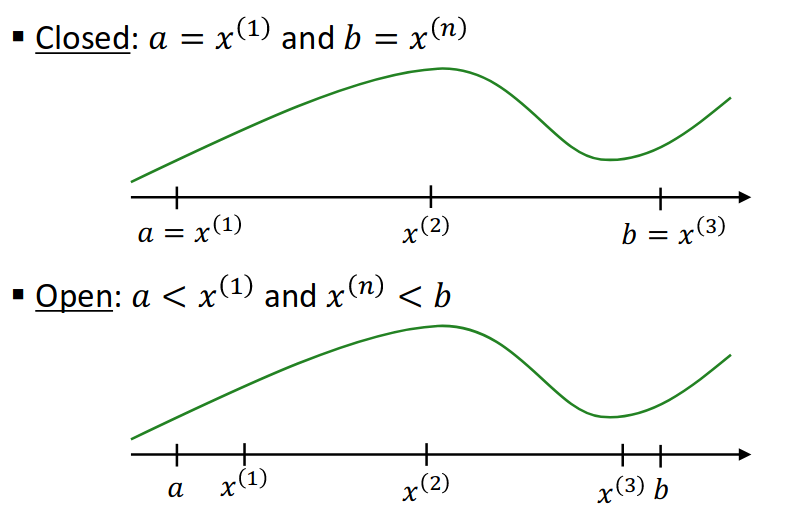
\includegraphics[scale=0.30]{img/openvsclosedpoints.png}
\end{figure}

\subsection{Méthode de Newton-Cotes}
Pour cette méthode, il faut $n$ points équidistants (fermés) $a = x^{(1)} < x^{(2)} < \ldots < x^{(n)} = b$ avec $$x^{(i)} = a + (i-1) * h$$
Où $h = \frac{b-a}{n-1}$ \newline
Ensuite, il faut utiliser l'interpolation de Lagrange pour approximer $f(x)$ (voir Slides 8.10) \newline
On obtient donc 
\begin{equation}
\int_a^bf(x)dx \approx \sum\limits_{i=1}^nf(x^{(i)})h\int_1^n \frac{\prod_{j \neq i} (t-j)}{\prod_{j \neq i}(i-j)}dt
\end{equation}

\subsubsection{Précision}
Pour $n$ points, $\sum\limits_{i=1}^nf(x^{(i)}\phi_i(x)$ est un polynôme de degré $n-1$. Du coup, pour $n = 2$, on peut intégrer $f(x)$ si et seulement si $f(x)$ est un polynôme de degré $\leq 1$. On a donc \newline
\textbf{Newton-Cotes avec} $n=2$ $\Longrightarrow$ \textbf{degré de précision} $=1$ \newline
Noter que si $f(x)$ est un polynôme de degré $1$, il suffit d'un point $x^{(1)} = \frac{a+b}{2}$ avec $\phi_1(x) = x$ et on obtient le même résultat que pour $n=2$ (Voir Slides 8.14) \newline
De manière générale : \textbf{La méthode de Newton-Cotes avec } $n$ \textbf{points et avec } $n+1$ \textbf{points à le même degré de précision } $n$ \textbf{si } $n$ \textbf{est pair.}

\subsubsection{Marge d'erreur}
L'erreur d'intégration est de 
\begin{equation}
|E| \leq \frac{M_n}{n!} |\int_a^b  \prod\limits_{i=1}^n (x - x^{(i)}) dx|
\end{equation} 
avec $M_n = \max\limits_{x \in [a,b]} |f^{(n)}(x)|$ 
\newline
(Voir Slides 8.16 8.17)

\subsubsection{Méthode trapézoïdale}
\label{intnum_trap}
La méthode trapézoïdale est un autre nom pour dire méthode de \textbf{Newton-Cotes} pour $n=2$.
\begin{figure}[!ht]
\centering
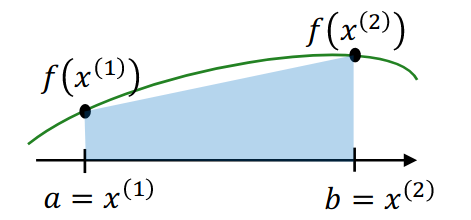
\includegraphics[scale=0.40]{img/trapezoidal.png}
\end{figure}
Où
\begin{itemize}
    \item[-] $h = b-a$ 
    \item[-] $\alpha_1 = \alpha_2 = \frac{1}{2}$
    \item[-] $\omega_1 = \omega_2 = \frac{b-a}{2}$
\end{itemize}
La méthode trapézoïdale approxime l'intégrale comme ceci:
\begin{equation}
    \int_a^b f(x)dx \approx (b-a) \frac{f(a) + f(b)}{2}
\end{equation}

\subsubsection{Méthode de Simpson}
\label{intnum_simpson}
La méthode de \textbf{Simpson} est un autre nom pour dire méthode de \textbf{Newton-Cotes} pour $n=3$.
\begin{figure}[!ht]
\centering
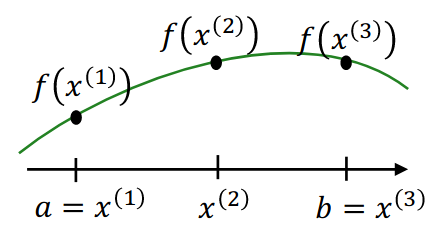
\includegraphics[scale=0.30]{img/simpson.png}
\end{figure}
Où
\begin{itemize}
    \item[-] $h = \frac{b-a}{2}$
    \item[-] $\alpha_1 = \alpha_3 = \frac{1}{3}$, $\alpha_2 = \frac{4}{3}$
    \item[-] $\omega_1 = \omega_3 = \frac{b-a}{6}$, $\omega_2 = \frac{2(b-a)}{3}$
\end{itemize}

La méthode de Simpson permet donc de calculer une intégrale de la manière suivante :
\begin{equation} 
    \int_a^b f(x)dx \approx \frac{b-a}{6}(f(a) + 4f(\frac{b-a}{2}) + f(b))
\end{equation}

\subsection{Méthode de composition}
L'idée de la méthode de composition est 
\begin{enumerate}
    \item Diviser $[a,b]$ en $N-1$ intervalles identiques $a = x^{(1)} < x^{(2)} < \ldots < x^{(N)} = b$
    \item Appliquer la méthode de \textbf{Newton-Cotes} sur chaque intervalle $[x^{(1)}, x^{(2)}]$, $[x^{(2)}, x^{(3)}]$, $\ldots$ avec des $n$ et des $h$ très petits : $h = \frac{b-a}{(N-1)*(n-1)}$.
    \item $\int_a^b f(x)dx \approx \int_a^{x^{(2)}} + \int_{x^{(2)}}^{x^{(3)}} + \int_{x^{(N-1)}}^b$
\end{enumerate}
On a donc un nombre total de points qui est égal à $(N-1)(n-1) + 1$ \newline
Voici un exemple de la méthode pour $N=3$ et $n=2$
\begin{figure}[!ht]
\centering
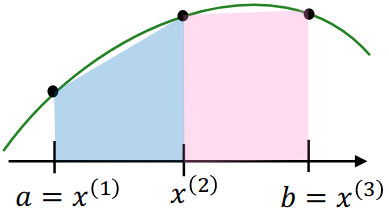
\includegraphics[scale=0.50]{img/ex_methodecomposition.png}
\end{figure}

\subsection{Méthode d'intégration adaptative}
Vu que l'erreur d'intégration dépend de $f^{(n)}(x)$ et que $f^{(n)}(x)$ peut varier beaucoup dans l'intervalle $x \in [a,b]$, on peut essayer de varier $h$ seulement là où on en a besoin au lieu de choisir des petits intervalles $h$ partout.
\begin{figure}[!ht]
\centering
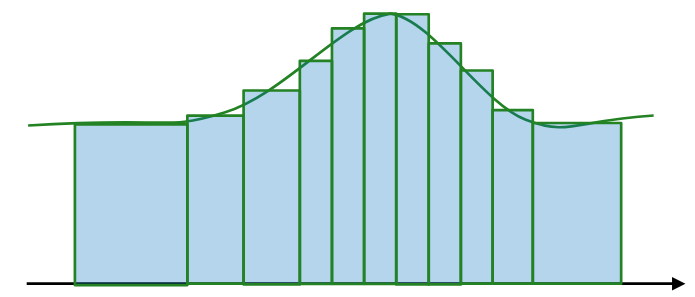
\includegraphics[scale=0.35]{img/adaptative_integration.png}
\end{figure}

\subsubsection{Algorithme général}
\begin{enumerate}
    \item Diviser l'intervalle $[a,b]$ en $N-1$ intervalles identiques aux points $a = x^{(1)} < x^{(2)} < \ldots < x^{(N)} = b$
    \item Pour chaque intervalle $[r,s]$:
    \begin{enumerate}
        \item Calculer $I_1 \approx \int_r^s$ en utilisant \emph{Newton-Cotes} avec des $n$ petits.
        \item Estimer l'erreur de $I_1$
        \item Si l'erreur est trop grande, diviser l'intervalle $[r,s]$ en deux intervalle plus petits ($[r,t]$ et $[t,s]$ avec $t = \frac{r+s}{2}$ et répéter l'étape 2. \newline
        \item Si l'erreur est acceptable, on prend $I_1$ comme estimation de $\int_r^s$.
    \end{enumerate}
\end{enumerate}
La question est donc : \textbf{comment estimer l'erreur à l'étape 2 ?}

\subsubsection{Algorithme avec "speculative splitting"}
\begin{enumerate}
    \item Diviser l'intervalle $[a,b]$ en $N-1$ intervalles identiques aux points $a = x^{(1)} < x^{(2)} < \ldots < x^{(N)} = b$
    \item Pour chaque intervalle $[r,s]$:
    \begin{enumerate}
        \item Calculer $I_1 \approx \int_r^s$ en utilisant \emph{Newton-Cotes} avec des $n$ petits.
        \item Calculer $I_2 = \int_r^t + \int_t^s$ avec $t = \frac{r+s}{2}$
        \item Comparer $I_1$ et $I_2$ :
        \begin{itemize}
            \item[-] Si $|I_1 - I_2| < \tau$, alors garder $I_2$ pour l'estimation de $\int_r^s$
            \item[-] Sinon, répéter l'étape 2 pour les sous-intervalles $[r,t]$ et $[t,s]$.
        \end{itemize}
    \end{enumerate}
\end{enumerate}
$\tau$ est une constante d'erreur limite choisie arbitrairement.

\subsection{Caractéristiques}
\begin{enumerate}
    \item Peut être implémenté très facilement récursivement
    \item Il est possible de commencer avec un seul intervalle $[a,b]$ à l'étape 1 mais il y a un risque de ne pas repérer les variations de $f$ si $n$ est petit. \newline
	\begin{figure}[!ht]
	\centering
    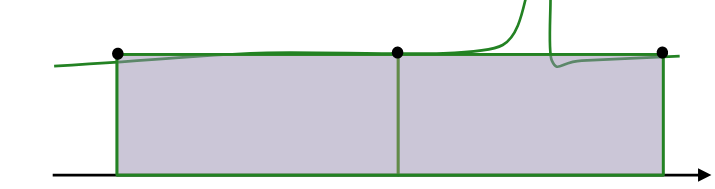
\includegraphics[scale=0.35]{img/adaptative_integration_remark2.png}
	\end{figure}
    \item Il faudrait s'arrêter lorsque les intervalles deviennent trop petits, sinon, l'arrondi des erreurs est trop grand.
\end{enumerate}

\subsection{Quadrature de Gauss-Legendre}
La formule générale de la quadrature est 
\begin{equation}
\int_a^b f(x)dx \approx \sum\limits_{i=1}^n \omega_i f(x^{(i)})
\end{equation}
Dans la méthode de Gauss-Legendre, les points $x^{(i)}$ ne sont pas équidistants. En choisissant les poids $\omega_i$ et les points $x^{(i)}$, on peut arriver à obtenir un degré de précision de $2n-1$. \newline
Trouver $\omega_i$ et $x^{(i)}$ nécessite des calculs compliqués (il existe des tables pour ces valeurs). Si on connait les $\omega_i$ et $x^{(i)}$ dans l'intervalle $[-1,1]$, on peut utiliser la formule 
\begin{equation}
    \int_a^b f(x) = \frac{b-a}{2} \sum\limits_{i=1}^n \omega_i f(\frac{b-a}{2}x^{(i)} + \frac{a+b}{2})
\end{equation}

\section{Dérivation numérique}

\subsection{One-sided differencing}
Graphiquement, l'approximation de la dérivée $f^{'}(x)$ est représentée comme ceci :
\begin{figure}[!ht]
\centering
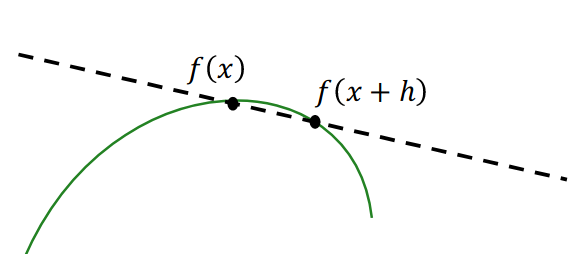
\includegraphics[scale=0.35]{img/geo_int_diff.png}
\end{figure}

\subsubsection{One-sided forward differencing}
\label{onesidedfd}
On peut approximer une dérivée avec le \textbf{one-sided forward differencing} comme ceci :
\begin{equation}
f^{'}(x) \approx \frac{f(x+h) - f(x)}{h}
\end{equation}
Pour un $h$ très petit. Il peut être montré (Voir Slides 9.5) que l'erreur de l'approximation est $-\frac{h}{2}f^{''}(\xi)$. Cette approximation est une méthode du premier ordre car l'erreur est en $O(h)$.

\subsubsection{One-sided backward differencing}
Une autre manière d'approximer une dérivée est la méthode de \textbf{one-sided backward differencing} : 
\begin{equation}
f^{'}(x) \approx \frac{f(x) - f(x-h)}{h}
\end{equation}
\subsection{Two-sided centered differencing}
Si on utilise les points $f(x-h)$ et $f(x+h)$ pour approximer $f^{'}(x)$, on obtient
\begin{equation}
f^{'}(x) \approx \frac{f(x+h) - f(x-h)}{2h}
\end{equation}
Graphiquement, cela revient à cela :
\begin{figure}[!ht]
\centering
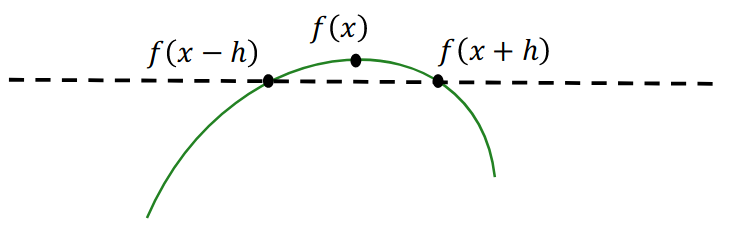
\includegraphics[scale=0.30]{img/two_sided_diff.png}
\end{figure}
On peut donc constater que notre erreur est maintenant de $O(h^2)$, on a donc une approximation du second ordre. \textbf{Attention !} Vu que $h$ est très petit, $h^2$ est encore plus petit que $h$ ! (Voir Slides 9.7)

\subsection{Higher differentiation}
On peut obtenir les dérivées d'ordre supérieur d'une manière très similaire. Pour trouver $f^{''}(x)$ on peut faire 
\begin{equation}
f^{''}(x) \approx \frac{f(x+h) - 2f(x) + f(x-h)}{h^{2}}
\end{equation}
avec une erreur du second ordre de $-\frac{h^2}{12}(f(^{''''}(\xi)))$.

\subsection{Extrapolation de Richardson}
Si on prend la formule du polynôme de Taylor, on peut écrire 
$$f^{'}(x) = D(h) + h^2e_2 + h^4e_4 + \ldots$$ avec $$D(h) = \frac{f(x+h) - f(x-h)}{2h}, e_2 = \frac{f^{'''}(x)}{12}, e_4 = \frac{f^{'''''}(x)}{60}\ldots$$
L'extrapolation de Richardson améliore l'ordre de l'erreur de $O(h^2)$ à $O(h^4)$ parce que les termes s'annulent (Faute de frappe sur le Slide 9.12) \newline
Il est très facile d'obtenir des approximations d'ordre supérieur avec l'extrapolation de Richardson, il suffit de répéter les étapes : \newline
On définit 
$$S(h) = \frac{-f(x+2h) + 8f(x+h) -8f(x-h) + f(x-2h)}{12h}$$
et on obtient 
$$f^{'}(x) = \frac{16S(h) - S(2h)}{16-1} + O(h^6)$$
La méthode fonctionne pour d'autres problèmes (par exemple : \emph{l'intégration numérique}), il est seulement nécessaire que la structure de l'erreur soit connue. (Par exemple : $f^{'}(x) = D(h) + h^2e_2 + h^4e_4 + \ldots$)

\subsubsection{Estimation d'erreur plus réaliste}
On ne peut pas utiliser des $h$ trop petits (Exemple : $10^{-100}$ car les ordinateurs ne sont pas capables de représenter tous les nombres. \newline
Au lieu d'utiliser $f^{'}(x) = \frac{f(x+h) - f(x-h)}{2h} - \frac{h^2}{6}f^{'''}(\xi)$, il est préférable d'utiliser
\begin{equation}
f^{'}(x) = \frac{f(x+h) - f(x-h)}{2h} + \frac{\epsilon}{2h} - \frac{h^2}{6}f^{'''}(\xi)
\end{equation}
Où $\epsilon$ est l'erreur machine de $f(x+h) - f(x-h)$ \newline
Pour les variable \emph{double} du IEEE, l'erreur machine est égale à $\mu = 2.2 * 10^{-16}$. On a donc $|\epsilon| \leq \mu(|f(x+h)| + |f(x-h)|)$. \newline
On peut estimer les bornes de l'erreur avec 
\begin{equation}
E(h) = \frac{\epsilon}{2h} - \frac{h^2}{12} f^{'''}(\xi) \leq \frac{\mu}{h}M_1 + \frac{h^2}{6}M_2
\end{equation}
Où $M_1 = \max|f(z)|$ et $M_2 = \max|f^{'''}(z)|$ pour $z \in [x-h, x+h]$ \newline
Pour un $h$ trop petit, l'erreur théorique ($\frac{h^2}{6}f^{'''}(x)$) est trop grande, tandis que pour un $h$ trop grand, l'erreur machine ($\frac{\mu}{h}|f(x)$) devient trop grande. \newline
Pour choisir un $h$ optimal, il faut résoudre l'équation $E^{'}(h) = 0$, ce qui donne 
$$h_{optimal} = (\frac{3\mu|f(x)|}{|f^{'''}(x)|})^{1/3}$$
En pratique, on n'utilise un $h$ optimal que lorsque c'est vraiment nécessaire (puisqu'il faut le calculer à la main

\section{Equations non-linéaires}

\subsection{Méthode de Bisection}
On a vu que résoudre des systèmes linéaires est quelque chose de plutôt facile, mais si on veut résoudre un système non-linéaire (Par exemple : $x^2 + e^{\cos x} - 3 = 0$, il faut trouver les racines de ce système ($f(x^{*}) = 0$). Jusqu'ici, la plupart des méthodes qu'on a vues sont des méthodes itératives qui ne convergent pas toujours vers la solution. \newline
Pour trouver une \emph{racine}, et si la fonction est continue, on peut utiliser le \textbf{Théorème des valeurs intermédiaires}: \newline
$\forall u $ avec $f(a) < u < f(b)$ ou bien $ f(b) < u < f(a)$, il existe $z \in [a,b]$ tel que $f(z) = u$. \newline
A partir de là, on peut en déduire que si on a deux valeurs $l$ et $r$, avec $f(l) * f(r) < 0$, alors $f(x)$ possède une racine $x^{*} \in [l,r]$. Ce qui nous donne l'algorithme de \textbf{bisection}.
On peut estimer l'erreur relative de l'algorithme de \textbf{bisection} à l'itération $k$ avec 
\begin{equation}
E_k = |x_k - x^* | < \frac{|r_k - r_l|}{2}
\end{equation} 
Puisqu'on divise l'intervalle en deux à chaque itération, l'erreur est réduite de moitié à chaque itération : $E_{k+1} = \frac{1}{2}E_k$

\subsection{Fixed point iteration}
Pour obtenir une meilleure convergence, on peut poser $f(x^*) + x^* = x^*$ au lieu de $f(x^*) = 0$. De manière générale : une valeur $x^*$ telle que $g(x^*) = 0$ est appelée le \emph{fixed point} de $g(x)$. \newline
Si on a une fonction $g(x) : [a,b] \in R$ avec un \emph{fixed point} \textbf{unique} $x^* \in [a,b]$, on peut prouver qu'il existe $c$ tel que 
\begin{equation}
|g(s) - g(t) \leq c|s-t|, \forall s,t \in [a,b]
\end{equation}
Si $c < 1$, alors l'itération $x_{k+1} = g(x_k)$ converge vers $x^*$ si on prend comme valeur initiale $x_0 \in [a,b]$ 

\subsection{Méthode de Newton(-Raphson) \label{newt_raphson}}
Si on sait que $f(x)$ est dérivable, on peut encore obtenir une meilleure convergence, grâce à la formule 
\begin{equation}
x_{k+1} = x_k - \frac{f(x_k)}{f^{'}(x_k)}
\end{equation}
L'itération converge de manière quadratique ($E_{k+1} = C*E_k^2$ où $C$ est une constante) vers $x^*$ si:
\begin{itemize}
    \item[-] La racine est unique
    \item[-] $f^{'}(x^*) \neq 0$ autour de la racine
    \item[-] $f^{''}(x)$ est continue
    \item[-] La valeur initiale $x_0$ est suffisamment proche de $x^*$
\end{itemize}
Pour trouver une valeur initiale $x_0$ correcte, on peut utiliser une méthode dont la convergence est garantie (par exemple : \emph{Bisection}).

\subsection{Méthode sécante \label{meth_secante}}
Lorsque $f^{'}(x_k)$ est inconnue/difficile à calculer, on peut réutiliser les calculs de l'itération précédente pour obtenir une itération de la forme 
\begin{equation}
x_{k+1} = x_k - \frac{f(x_k)(x_k - x_{k-1})}{f(x_k) - f(x_{k-1})}
\end{equation}
Puisque $f^{'}(x_k) \approx \frac{f(x_k) - f(x_{k-1})}{x_k - x_{k-1}}$. La convergence n'est alors plus quadratique mais est $E_{k+1} = C*E_k^{1.618034}$

\subsection{Méthode de Newton pour des systèmes non-linéaires}
Pour résoudre un système non-linéaire avec la méthode de \textbf{Newton-Rapĥson}, on utilise 
\begin{equation}
X_{k+1} = X_k - (J_F(X_k))^{-1}F(X_k)
\end{equation}
au lieu de $x_{k+1} = x_k - \frac{f(x_k)}{f^{'}(x_k)}$, où $J_F(X)$ est la matrice Jacobienne de $F$ : 
$$ J_F(X) = 
\begin{pmatrix}
\frac{\delta f_1}{\delta x_1}(X) & \frac{\delta f_1}{\delta x_n}(X) & \ldots & \frac{\delta f_1}{\delta x_n}(X) \\
\frac{\delta f_2}{\delta x_1}(X) & \frac{\delta f_2}{\delta x_2}(X) & \ldots & \frac{\delta f_2}{\delta x_n}(X) \\
\ldots & \ldots & \ldots & \ldots \\
\frac{\delta f_n}{\delta x_1}(X) & \frac{\delta f_n}{\delta x_2}(X) & \ldots & \frac{\delta f_n}{\delta x_n}(X) \\
\end{pmatrix}
$$
avec $\frac{\delta f_i}{\delta x_i}(x_1, \ldots, x_n) = \frac{d}{dt} f_i(x_1, \ldots, x_{j-1}, t, x_{j+1}, \ldots, x_n)|_{t=x_j}$ \newline
Au lieu de calculer $(J_F(X_k))^{-1}$ directement, il est plus efficace de résoudre le système $F_F(X_k)Y = F(X_k)$. Cette méthode est cependant très coûteuse, puisqu'il faut calculer la matrice Jacobienne à chaque itération.

\section{Problèmes à valeurs initiales}

\subsection{Equations différentielles ordinaires (ODE)}
La forme générale d'une \textsc{ODE} (\emph{explicite}) d'ordre $1$ est :
$$f^{'}(x) = F(x, f(x))$$,
où il faut trouver $f(x)$ pour la fonction $F$.

\subsection{Problèmes à valeurs initiales (IVP)}
La forme générale d'une \textsc{IVP} d'ordre $1$ est :
$$f^{'}(x) = F(x, f(x))$$
$$f(a) = v$$
Où il faut trouver $f(x)$ pour la fonction $F$ avec comme valeur initiale $f(a) = v$. \newline
Les problèmes à valeurs initiales n'ont pas toujours de solutions uniques (\emph{ni de solutions tout court}), il est également possible qu'il y ait une infinité de solutions  (\emph{familles de solutions}).

\subsubsection{Méthode Forward Euler}
\label{ivp_forward_euler}
En connaissant une IVP 
$$f^{'}(x) = F(x, f(x))$$
$$f(a) = v$$
La méthode de \textbf{Forward Euler} est une méthode \emph{explicite} qui tente d'approximer $f(x)$ avec des points équidistants : 
$$f(x_0), x_0 = a$$
$$f(x_1), x_1 = a+h$$
$$f(x_2), x_2 = a+2h$$
$$\ldots$$
Etant donné que le point de départ $f(x_0) = f(a) = v$ est connu, on peut calculer les $x_k$ avec la méthode de \textbf{one-sided forward differencing} (\ref{onesidedfd}). L'équation
\begin{equation}
f(x_{i+1}) = hF(x_i, f(x_i)) + f(x_i) + \frac{h^2}{2}f^{''}(\xi_{i+1})
\end{equation}
permet de trouver une procedure itérative pour approximer les valeurs de $f(x_i)$ aux points $x_i$.
On commence par calculer 
$$f_0 = f(a) = v$$
Puis on calcule
$$f_{i+1} = hF(x_i, f_i) + f_i$$
Pour $i = 1, 2, 3, \ldots$, et on espère que $f(x_{i+1}) \approx f_{i+1}$

\paragraph{Erreur locale :} 
A chaque étape, on fait $f(x_{i+1}) = f_{i+1} = hF(x_i, f_i) + f_i$. On a donc une erreur égale à $\frac{h^2}{2}f^{''}(\xi_{i+1})$ pour chaque itération. (Cette erreur est appelée \emph{localized truncation error} de l'étape $f_i$ à $f_{i+1}$).

\paragraph{Erreur globale :} 
$$e_{i+1} = e_i + e_i h\frac{\delta F}{\delta f}|_{x_i, \zeta_i} + \frac{h^2}{2}f^{''}(\xi_{i+1})$$
On peut la réécrire comme $$e_{i+1} = e_i a_i + l_{i+1}$$
où
$$l_{i+1} = \frac{h^2}{2} f^{''}(\xi_{i+1})$$
$$a_i = 1 + h \frac{\delta F}{\delta f}|_{(x_i, \zeta_i)}$$
$l_{i+1}$ est l'erreur locale en $O(h^2)$ et $a_i$ est en $O(h)$.
Une IVP est stable avec cette méthode si $|a_i| < 1$. Vu la formule de $|a_i|$, on peut en conclure que les systèmes $\frac{\delta F}{\delta f}|_{(x_i, \zeta_i)} > 0$ sont instables puisque l'erreur grandit à chaque itération, peu importe le $h$ choisi. A l'inverse, si $\frac{\delta F}{\delta f}|_{(x_i, \zeta_i)} < 0$, l'IVP est alors stable. Si on choisit $h < - \frac{2}{\frac{\delta F}{\delta f}|_{(x_i, \zeta_i)}}$, alors l'erreur va converger vers $0$.

\subsubsection{Méthode Backward Euler}
La méthode \textbf{backward Euler} est une méthode \emph{implicite}, qui utilise le \emph{one-sided backward differencing} (au lieu de \emph{one-sided forward differencing} pour le \emph{forward Euler}). Ce qui donne 
\begin{equation}
(x_{i+1}) \approx f_{i+1} := hF(x_{i+1}, f_{i+1}) + f_i
\end{equation}
A chaque itération, on aura donc besoin de résoudre le système 
\begin{equation} 
f_{i+1} = hF(x_{i+1}, f_{i+1}) + f_i
\end{equation}
Donc, pour calculer $x_{i+1}$, il nous faut une approximation de $x_{i+1}$. On peut obtenir cette approximation de plusieurs manières différentes.
\begin{itemize}
    \item[-] Si on connait la dérivée de la fonction, on peut utiliser la méthode de \textbf{Newton(-Raphson)} \ref{newt_raphson}
    \item[-] Si on ne la connait pas, on peut utiliser la \textbf{méthode sécante} \ref{meth_secante}.
\end{itemize}
(L'examen de Janvier 2019 demandait d'implémenter les deux)

\paragraph{Erreur locale :}
$$l_i = - \frac{h^2}{2} f^{''}(\xi_{i+1})$$
Comme pour la méthode \emph{forward Euler}, la méthode \textbf{backward Euler} est stable si $|a_i| < 1$ sauf qu'ici 
\begin{equation}
a_i = \frac{1}{1 - h \frac{\delta F}{\delta f}|_{(x_i, \xi_i)}}
\end{equation}
Ce qui veut dire que le système est stable pour n'importe quel $h$ si $\frac{\delta F}{\delta f}|_{(x_i, \xi_i)} < 0$

\subsubsection{Méthode trapézoïdale}
Si on définit un IVP comme 
$$f(x_{i+1}) = f(x_i) + \int_{x_i}^{x_{i+1}} f^{'}(x)dx$$
On peut utiliser la méthode d'\textbf{intégration trapézoïdale} (\ref{intnum_trap}) pour approximer l'intégrale 
$$\int_{x_i}^{x_{i+1}} f^{'}(x)dx = (x_{i+1} - x_i) \frac{f^{'}(x_i) + f^{'}(x_{i+1})}{2} + O(h^3)$$
Sachant que $f^{'}(x) = F(x, f(x))$ et que $h = x_{i+1} x_i$, on peut en obtenir l'équation équivalente :
$$f(x_{i+1}) = f(x_i) + h \frac{F(x_i, f(x_i)) + F(x_{i+1}, f(x_{i+1}))}{2} + O(h^3)$$
Ce qui permet d'obtenir la formule d'itération
\begin{equation}
f_{i+1} = h \frac{F(x_i, f_i) + F(x_{i+1}, f_{i+1})}{2} + f_i
\end{equation}
La méthode trapézoïdale a comme caractéristiques :
\begin{itemize}
    \item[-] Cette méthode est implicite et inconditionnellement stable
    \item[-] Meilleure approximation que \emph{backward Euler} mais plus long à calculer
    \item[-] Erreur locale en $0(h^3)$
    \item[-] Erreur globale en $0(h^2)$
\end{itemize}

\section{Plus de problèmes à valeurs initiales}

\subsection{Méthodes de Runge-Kutta}
Les méthodes \textbf{Runge-Kutta} sont basées sur l'observation suivante : 
$$f(x_{i+1}) = f(x_i) + \int\limits_{x_i}^{x_{i+1}}f^{'}(x)dx = f(x_i) + \int\limits_{x_i}^{x_{i+1}} F(x, f(x))dx$$
Bien que $f(x)$ soit inconnue, on peut tenter de l'approximer grâce à l'intégration numérique (\ref{intnum})
\subsubsection{Méthode de Heun}
La méthode de Heun utilise la méthode \textbf{trapézoïdale} \ref{intnum_trap}, mélangée avec la méthode de \textbf{Forward Euler} \ref{ivp_forward_euler} (Explications Slides 12.1.3). Ce qui donne une formule \emph{explicite} : 
\begin{equation}
f_{i+1} := f_i + \frac{h}{2}(K_1 + K_2)
\end{equation}
Où
$$K_1 = F(x_i, f_i)$$
$$K_2 = F(x_{i+1}, f_i + hK_1)$$

\paragraph{Erreur locale :} 
$O(h^3)$
\paragraph{Erreur globale :} 
$O(h^2)$
\paragraph{Condition de stabilité :} 
Pareille que celle de \textbf{Forward Euler} puisque la méthode de \textbf{Heun} utilise cette méthode.

\subsubsection{Méthode de Runge-Kutta classique (\textbf{RK4})}
La méthode \textbf{RK4} est similaire par rapport à la méthode de \emph{Heun} dans le sens où elle utilise aussi \textbf{Forward Euler}, sauf qu'au lieu d'utiliser la méthode trapézoïdale, elle utilise l'approximation de Simpson \ref{intnum_simpson} : 
\begin{equation}
f_{i+1} = f_i + \frac{h}{6} (K_1 + 2K_2 + 2K_3 + K_4)
\end{equation}
Où
$$K_1 = F(x_i, f_i)$$
$$K_2 = F(x_i + \frac{h}{2}, f_i + \frac{h}{2}K_1)$$
$$K_3 = F(x_i + \frac{h}{2}, f_i + \frac{h}{2}K_2)$$
$$K_4 = F(x_{i+1}, f_i + hK_3)$$

\paragraph{Erreur locale :} 
$O(h^5)$
\paragraph{Erreur globale :} 
$O(h^4)$

\subsection{Systèmes de problèmes à valeurs initiales}
Un système d'IVP correspond à
$$f_1^{'}(x) = F(x, f_1(x), \ldots, f_n(x))$$
$$\ldots$$
$$f_n^{'}(x) = F(x, f_1(x), \ldots, f_n(x))$$
Avec comme valeurs initiales :
$$f_1(a) = v_1$$
$$\ldots$$
$$f_n(a) = v_n$$
Pour résoudre ce type de systèmes, on peut appliquer directement les méthodes pour résoudre une seule IVP (Par exemple : \textbf{Forward Euler} \ref{ivp_forward_euler})

\subsection{Problèmes à valeurs initiales d'ordre supérieur}
Un IVP d'ordre $n$ a comme forme générale :
$$f^{(n)} = F(x, f(x), f^{'}(x), \ldots, f^{(n-1)}(x))$$
$$f(a) = v_0$$
$$f^{'}(a) = v_1$$
$$\ldots$$
$$f^{n-1}(a) = v_{n-1}$$

\subsubsection{Transformer un IVP d'ordre supérieur}
Un IVP d'ordre supérieur à $1$ peut être modélisé comme un système d'IVP du premier ordre. Par exemple pour un IVP d'ordre $2$ : 
$$f^{''}(x) = F(x, f(x), f^{'}(x))$$
$$f(a) = v_0$$
$$f^{'} = v_1$$

On peut transformer le système en posant $f_1(x) := f(x)$ et $f_2(x) := f^{'}(x)$, ce qui nous donne un système du premier ordre, dont les solutions sont les mêmes :
$$f_1^{'}(x) = f_2(x)$$
$$f_2^{'}(x) = F(x, f_1(x), f_2(x))$$
$$f_1(a) = v_0$$
$$f_2(a) = v_1$$


\subsubsection{Généralisation de la résolution d'IVP d'ordre supérieur}
Un IVP d'ordre $n$
$$f^{(n)}(x) = F(x, f(x), f^{'}(x), \ldots, f^{(n-1)}(x)$$
$$f(a) = v_0$$
$$\ldots$$
$$f^{(n-1)}(a) = v_{n-1}$$

Peut être transformée en système d'IVP du premier ordre, en posant $f_i = f^{(i-1)}(x)$ : 

$$f_1^{'}(x) = f_2(x)$$
$$f_2^{'}(x) = f_3(x)$$
$$\ldots$$
$$f_n^{'}(x) = F(x, f_1(x), f_2(x), \ldots, f_n(x))$$
$$f_1(a) = v_0$$
$$f_2(a) = v_1$$
$$\ldots$$

\end{document}
